% ---------------------------------
\mysec{Winkel an Geradenkreuzungen}
% ---------------------------------
\begin{minipage}[c]{0.45\linewidth}
  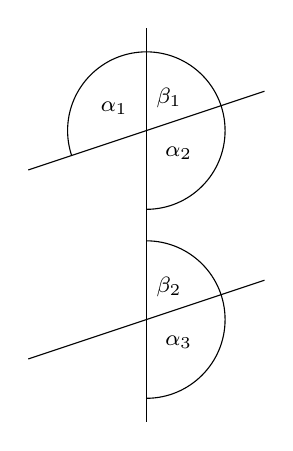
\begin{tikzpicture}
    \draw (1.5, 0.0) -- (1.5, 5.0);
    \draw (0.0, 3.2) -- (3.0, 4.2);
    \draw (0.0, 0.8) -- (3.0, 1.8);
    % Winkel oben
    \begin{scope}
      \clip (1.5, 3.7) --
            (0.0, 3.2) --
            (0.0, 5.0) --
            (3.0, 5.0) --
            (3.0, 1.8) --
            (1.5, 1.8) -- cycle;
      \draw (1.5, 3.7) circle (1cm);
      \node[shift=(145:5mm)] at (1.5, 3.7) {{\footnotesize$\alpha_{1}$}};
      \node[shift=(325:5mm)] at (1.5, 3.7) {{\footnotesize$\alpha_{2}$}};
      \node[shift=( 55:5mm)] at (1.5, 3.7) {{\footnotesize$\beta_{1}$}};
    \end{scope}
    % Winkel unten
    \begin{scope}
      \clip (1.5, 0.0) --
            (1.5, 2.5) --
            (3.0, 2.5) --
            (3.0, 0.0) -- cycle;
      \draw (1.5, 1.3) circle (1cm);
      \node[shift=(325:5mm)] at (1.5, 1.3) {{\footnotesize$\alpha_{3}$}};
      \node[shift=( 55:5mm)] at (1.5, 1.3) {{\footnotesize$\beta_{2}$}};
    \end{scope}
  \end{tikzpicture}
  \vspace*{\baselineskip}
\end{minipage}%
\hfill
\begin{minipage}[c]{0.54\linewidth}
  Nebenwinkel:
  \formrow{\alpha_{1}+\beta_{1}=180^{\circ}}

  Scheitelwinkel:
  \formrow{\alpha_{1}=\alpha_{2}}

  Stufenwinkel:
  \formrow{\beta_{1}=\beta_{2}}

  Wechselwinkel:
  \formrow{\alpha_{1}=\alpha_{3}}
\end{minipage}%

